\section{Analysis}

\begin{frame}
    \frametitle{Protocols}

    XMPP (mainly used by IM and VoIP) traffics experience longer latency than HTTP(s).

    \vskip 1em
    \centering
    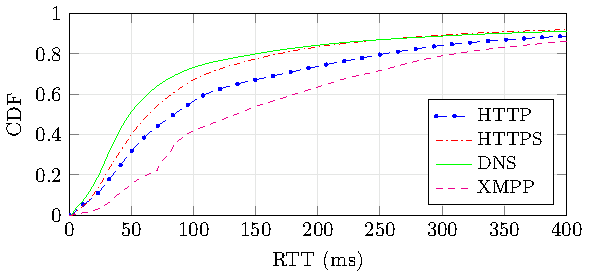
\includegraphics[width=.65\textwidth]{fig/port_performance.pdf}

    % 5222, 5223 and 5224 are used by XMPP, which is a common protocol for IM and VoIP services.
\end{frame}

% \begin{frame}
%     \setcounter{footnote}{0}
%     \frametitle{DNS Performance}

%     % We know DNS is a criticle part of todays internet, and it's performance has great impacts on the QoE
%     Users using DNS server that are located on different countries\footnote{servers deployed IP Anycast are considered ``diff country'' in this chapter} experience longer latency to app servers. This suggests the need for IP Anycasting.

%     \vskip 1em
%     \begin{columns}
%         \begin{column}{.5\textwidth}
%             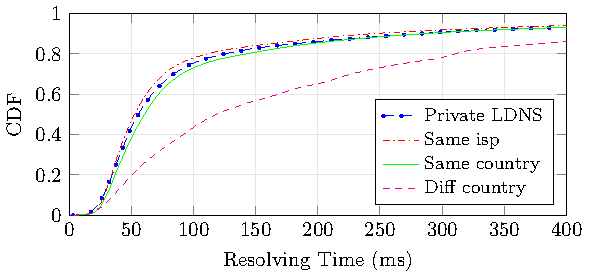
\includegraphics[width=\textwidth]{../fig/dns_performance.eps}
%         \end{column}

%         \begin{column}{.5\textwidth}
%             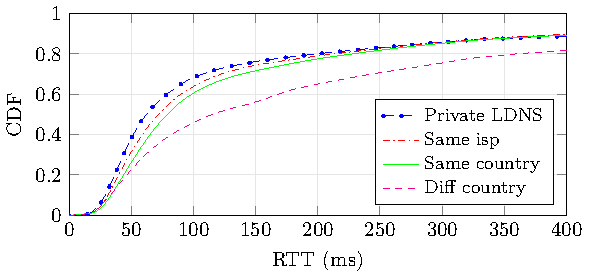
\includegraphics[width=\textwidth]{../fig/dns_overall.eps}
%         \end{column}
%     \end{columns}
% \end{frame}

% \begin{frame}
%     \setcounter{footnote}{0}
%     \frametitle{IP Anycast}
%     We found that apps with DNS redirections still benefits from IP Anycast.
%     The Anycast IP are identified using the the list conducted by iGreedy.\footnote{https://anycast.telecom-paristech.fr/dataset/}
%     We use rlm() from R package MASS with default parameters to perform robust regression.

%     \vskip 1em
%     \centering
%     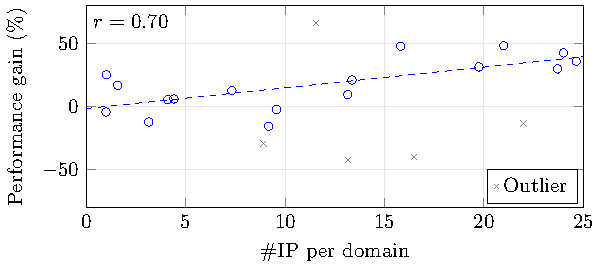
\includegraphics[width=.65\textwidth]{../fig/anycast_nip_per_domain.pdf}
% \end{frame}

\begin{frame}
    \setcounter{footnote}{0}
    \frametitle{DNS Redirection and IP Anycast\footnote{Identified using iGreedy: https://anycast.telecom-paristech.fr/dataset/} performance}

    \begin{itemize}
        \setlength{\itemsep}{1.4em}
        \item Using DNS servers located in a different country could increase the median latency by about 50\%.
        \item Domains that already deployed DNS redirections could still benefit from IP Anycast.
    \end{itemize}
\end{frame}

% \begin{frame}
%     \frametitle{Application Servers}
%     \centering
%     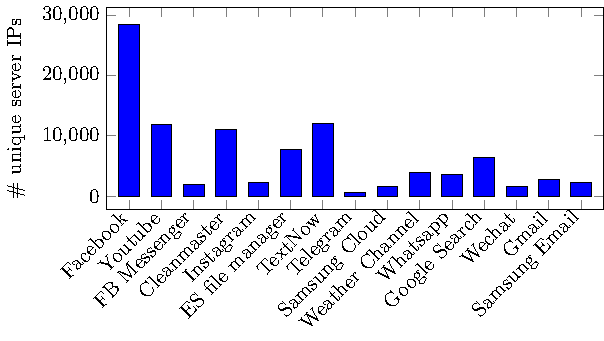
\includegraphics[width=.65\textwidth]{../fig/server_number.pdf}
% \end{frame}

\begin{frame}
    \setcounter{footnote}{0}
    \frametitle{Advertisement Servers\footnote{Identified using EasyList: https://easylist.to/}}

    \begin{itemize}
        \setlength{\itemsep}{1.4em}
        \item For some apps more than 50\% of traffic goes to advertisement providers.
        \item However, these traffic often has longer RTTs than the apps' own API servers.
        \item Companies with decent CDN deployments could improve the loading time by caching ads themselves.
    \end{itemize}

    % We found that many ads are slower than the api server. It suggests that companies with decent CDN deployments could improve the loading time by caching ads themselves.

    % \vskip .6em
    % \centering
    % 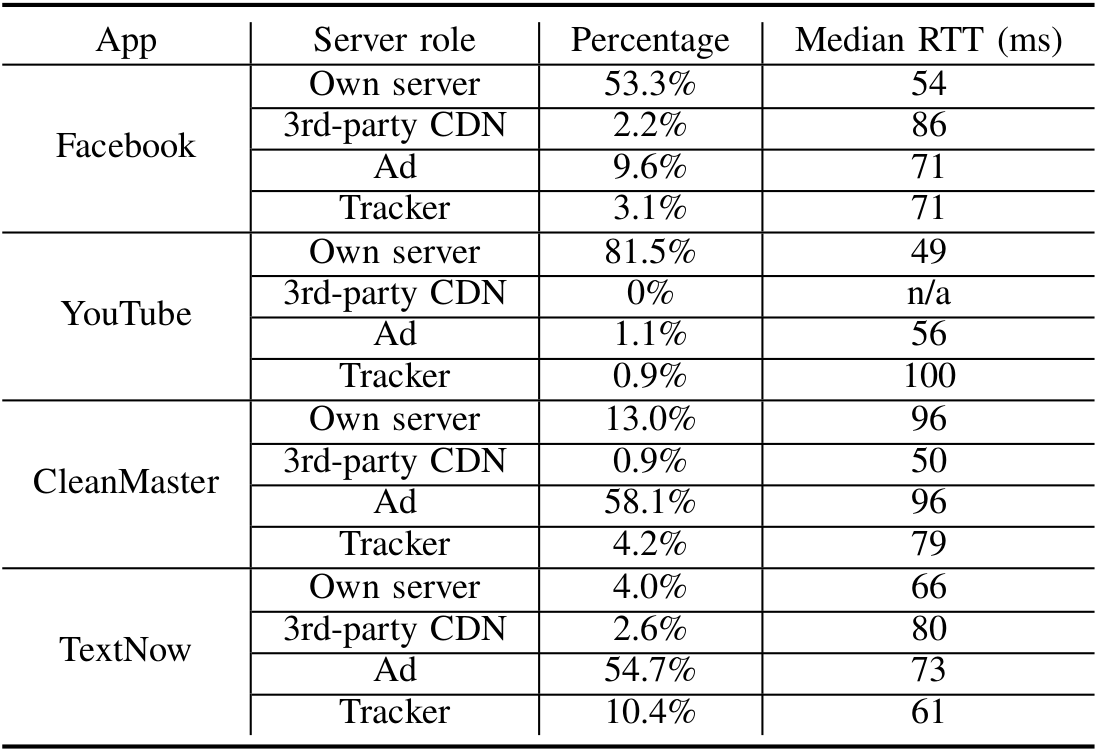
\includegraphics[width=.52\textwidth]{table.png}
\end{frame}
